\documentclass{ieeeaccess}

\usepackage{cite}
\usepackage{amsmath,amssymb,amsfonts}
\usepackage{algorithmic}
\usepackage{graphicx}
\usepackage{textcomp}
\def\BibTeX{{\rm B\kern-.05em{\sc i\kern-.025em b}\kern-.08em
		T\kern-.1667em\lower.7ex\hbox{E}\kern-.125emX}}

\usepackage{lineno,hyperref}
\usepackage{subfig}
\usepackage{graphicx}
\usepackage{rotating}
\usepackage{multirow}
\usepackage{enumerate}
\usepackage{longtable}
\usepackage{comment}


\usepackage{array}
%\newcolumntype{L}[1]{>{\raggedright\let\newline\\\arraybackslash\hspace{0pt}}m{#1}}
\newcolumntype{C}[1]{>{\centering\let\newline\\\arraybackslash\hspace{0pt}}m{#1}}
%\newcolumntype{R}[1]{>{\raggedleft\let\newline\\\arraybackslash\hspace{0pt}}m{#1}}

\graphicspath{{./images/}}

\newtheorem{theorem}{Theorem}

\begin{document}
\history{Date of publication xxxx 00, 0000, date of current version xxxx 00, 0000.}
\doi{10.1109/ACCESS.2017.DOI}

\title{Morphological Filter Detector for Image~Forensics~Applications}
\author{\uppercase{Giulia Boato}\authorrefmark{1}, \IEEEmembership{Member, IEEE},
\uppercase{Duc-Tien Dang-Nguyen}\authorrefmark{2}, \IEEEmembership{Member, IEEE} and \uppercase{Francesco G.B. De Natale}\authorrefmark{1},\IEEEmembership{Senior Member, IEEE}}
\address[1]{University of Trento, Italy (e-mail: giulia.boato@unitn.it; francesco.denatale@unitn.it)}
\address[2]{University of Bergen, Norway(e-mail: ductien.dangnguyen@uib.no)}
%\tfootnote{``This work was supported in part by ABC DEF GHI under Grant 123 456 789.''}

\markboth
{Boato \headeretal: Morphological Filter Detector for Image~Forensics~Applications}
{Boato \headeretal: Morphological Filter Detector for Image~Forensics~Applications}

\corresp{Corresponding author: Giulia Boato (e-mail: giulia.boato@unitn.it).}

\begin{abstract}
Mathematical morphology provides a large set of powerful non-linear image operators, widely used for feature extraction, noise removal or image enhancement. Although morphological filters might be used to remove artifacts produced by image manipulations, both on binary and graylevel documents, little effort has been spent towards their forensic identification. In a previous work \cite{de2017detecting}, a deterministic approach was proposed to detect erosion and dilation of binary images. In this paper we propose a non-trivial extension of such method that operates on grayscale images and is robust to image compression and other typical attacks. When the image is attacked the method looses its deterministic nature and uses a properly trained SVM classifier, using the original detector as a feature extractor. Extensive tests demonstrate that the proposed approach guarantees very high accuracy in filtering detection also after a high compression, and is also able to determine the adopted structuring element for moderate compression factors.
\end{abstract}

\begin{keywords}
Digital Image Forensics, Media Authentication, Morphological Filter Detection
%
%Enter key words or phrases in alphabetical order, separated by commas. For a list of suggested keywords, send a blank 
%e-mail to keywords@ieee.org or visit \underline
%{http://www.ieee.org/organizations/pubs/ani\_prod/keywrd98.txt}
\end{keywords}

\titlepgskip=-15pt

\maketitle

\section{Introduction}
\label{sec:intro}

In the last decade, researchers and practitioners in multimedia forensics have been developing a substantial body of knowledge and techniques targeted to the authentication of multimedia objects and their processing history recovery \cite{stamm_overview, farid_book, ho, piva_overview, sencar_book}. 
A recent trend tries to define universal detectors able to reveal manipulations independently from the type of processing applied, which could leverage media authentication in applications like journalism or social media analysis \cite{noiseprint}. 
On the other hand, many methods have been proposed to detect different types of forgeries, which is very relevant for diverse applications, in particular digital investigations - given that images, audio tracks and video sequences now play a crucial role in modern investigations where they often represent digital evidences to the court \cite{forlab} - and multimedia data phylogeny aiming at recovering and tracing back the life-cycle of an image or a video \cite{Bestagini2016, Dias2012, Oliveira2016, Costa2014}.

This broad class of specific manipulation detectors includes the identification of pasted regions \cite{cm2, cm3, cm4, spl2, spl3}, resizing \cite{fernando2017, PB-TIFS-2019}, re-compression \cite{PBPG2017-TIFS},  image enhancing \cite{shan2019robust}, inconsistencies in the geometry and illumination of the image due to possible manipulations \cite{geom1, geom2, phys1}, and various types of non-linear filtering (especially median) \cite{Bahrami2015, Cao2014, Cao2011, Fridrich2010, Tian2010, Yuan:2011, Liu2013, Huang2013, Shi2014, Wang2015, Pasquini2016-TIFS, gao2019robust}. 

In the context of non-linear filtering detection 
very little attention was given to morphological filters \cite{haas1967morphologie} often used in image processing for artifacts removal and image enhancement \cite{British2012} \cite{Maragos2004}. The detection of this kind of filtering is of interest in the context of both image phylogeny and specific tampering identification in legal scenarios, but could be very useful also to detect possible counter forensic attacks based on morphology, where such filters, very powerful in the removal of local noise, could be exploited at the end of the image manipulation process to cover other types of traces. 

In this paper we present a non trivial extension of a recent work \cite{de2017detecting} which introduced a deterministic detector of erosion and dilation in binary images. The proposed extension works on grayscale images by detecting morphological filters application in an accurate way both in uncompressed and compressed images. The method also allows for erosion versus dilation discrimination and in many cases also for the adopted structural element identification. 
Robustness against JPEG compression, noise addition and confusion with other types of filters is also tested on various datasets. 

The rest of the paper is organized as follows: Section~\ref{sec:theory} provides the theoretical background for the problem formulation; Section~\ref{sec:method} describes the proposed methodology for morphological filtering detection in uncompressed and compressed images; Section~\ref{sec:exp_setup} describes the experimental setup, datasets and scenarios adopted for testing and validation; Section~\ref{sec:experiments} details the experimental analysis and obtained results; finally, Section~\ref{sec:conclusions} reports some concluding remarks.   

\section{Theoretical formulation}
\label{sec:theory}
In this section we introduce the mathematical formulation of the problem, and we derive the proposed methodology for morphological filter detection. 

\subsection{Mathematical Formulation and Properties}
Mathematical morphology defines a set of nonlinear filters commonly employed in digital image processing to modify the local structural content of images. All the morphological filters are derived from the various combinations of two basic operators, \textit{erosion} and \textit{dilation}, and a kernel mask (or shortly, a kernel) called \textit{structuring element}, characterized by a shape, a size, and a reference point. The shape and the size of the kernel are responsible for the behavior of the operator on the image, while the reference point just defines the shift of the filtered image with respect to the original. The invention of such mathematical tools dates back to 1964 \cite{haas1967morphologie}, and was meant to the filtering of binary images for mineral studies. Later studies \cite{nakagawa1977note} led to the generalization of the theory to the case of grayscale images.

According to this theory, given a grayscale image $f(x,y)$ and a binary structuring element $B$, the two fundamental morphological operators, erosion and dilation, are respectivelly defined as:

\begin{equation} \label{eq:erode}
f \ominus B = min_B(f(x,y) \cap B_{xy})
\end{equation}
\begin{equation} \label{eq:dilate}
f \oplus B = max_B(f(x,y) \cap B_{xy})
\end{equation}

where $B_{xy}$ represents the structuring element (kernel) $B$ with the reference point centered at the coordinates $x,y$ of the image plane, while the intersection operations returns the subset of the image pixels overlapped with the 1s of $B$. In this respect, the basic grayscale operators are particular cases of rank-order filters, and behave very similarly to min-max and median operators, except for the shape of the mask.

\begin{figure}[h!]
	\centering
	\begin{tabular}{cc}
		\centering
		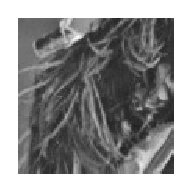
\includegraphics[scale=1.5]{original.eps} & 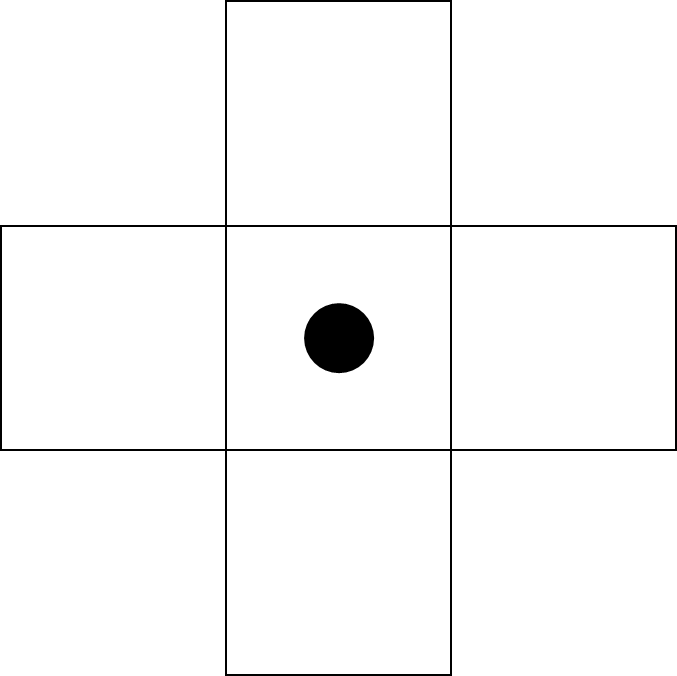
\includegraphics[scale=0.15]{mask.png} \\
		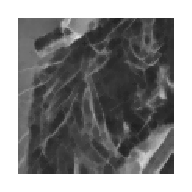
\includegraphics[scale=1.5]{eroded.eps} &  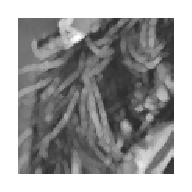
\includegraphics[scale=1.5]{dilated.eps} \\
	\end{tabular}
	\caption{Example of gray-scale erosion (bottom left) and dilation (bottom right) of an image detail (top left), using a cross-shaped structuring element (top right). The resulting patches show the effect of min and max operations: erosion produces a darker version of the original image eliminating small cross-shaped details, while dilation produces the opposite effect.}
\end{figure}

As in binary morphology, the composition of erosion and dilation allows defining more complex filters, among which the most common are the \textit{open} and \textit{close} operators, respectively defined as follows:

\begin{equation}
(f \circ B) = (f \ominus B) \oplus B
\end{equation}
\begin{equation}
(f \bullet B) = (f \oplus B) \ominus B
\end{equation}

Also the mathematical properties of morphological grayscale operators match the ones of the corresponding binary operators. Consequently, the theoretical background of \cite{de2017detecting} remains valid also for in the grayscale domain. In particular, the following properties are exploited in the construction of the proposed detector:

\begin{enumerate}[(i)]
	\item Translation invariance: the position of the reference point only affects the translation of the filtered image
	\item Dilation commutativity: $A\oplus B = B \oplus A$
	\item Associativity: a cascade of erosions (dilations) is equal to the erosion (dilation) with a mask generated by dilating each other the original masks
	\begin{equation}
	A \ominus B \ominus C = A \ominus (B \oplus C)
	\end{equation}
	\begin{equation}
	A \oplus B \oplus C = A \oplus (B \oplus C)
	\end{equation} 
	\item Open and close idempotence: iterating open and close with the same structural element does not produce additional changes in the image
	\begin{equation}
	A \circ B \circ B = A \circ B
	\end{equation}
	\begin{equation}
	A \bullet B \bullet B = A \bullet B
	\end{equation} 
\end{enumerate}

Additionally, it is easy to see that the two theorems introduced in \cite{de2017detecting} remain valid, since their demonstrations do not depend on Eq. \ref{eq:erode} and Eq. \ref{eq:dilate}, but only on the properties (i)-(iv), which hold also for grayscale images.

\begin{theorem}
	\label{theorem_1}
	Let $I' = I \ominus K$, then $I'\bullet K = I'$. Respectively, if $I' = I \oplus K$, then $I'\circ K = I'$.
\end{theorem}

\begin{theorem}
	\label{theorem_2}
	Let $I' = I \ominus K$, then $\forall M$ such that $\exists E | M \oplus E = K$, we have that $I' \bullet M = I'$. Respectively, if $I' = I \oplus K$, then $I' \circ M = I'$.
\end{theorem}

Theorem \ref{theorem_1} can be equivalently formulated in terms of series of erosion and dilation operators, according to the definition of open and close operators. Theorem \ref{theorem_2} extends the equality of Theorem \ref{theorem_1} to any kernel mask $M$ that can produce $K$ by dilation with an appropriate kernel $E$.

As an immediate consequence of the above theorems, an image dilated (eroded) with a given kernel $K$, will remain unchanged after applying an open (close) operator with the same element. This provides a simple test to detect a filtered image: apply an open (close) operator with a kernel $K$, if the image does not change, this means that it was previously dilated (eroded) with that kernel, otherwise it was not. The detection consists then in subsequently checking with the above procedure a set of possible masks. In \cite{de2017detecting}, a set of common kernels were proposed, characterized by some level of symmetry (see Figure \ref{fig:masks}).

\begin{figure}[!t]
	\centering
	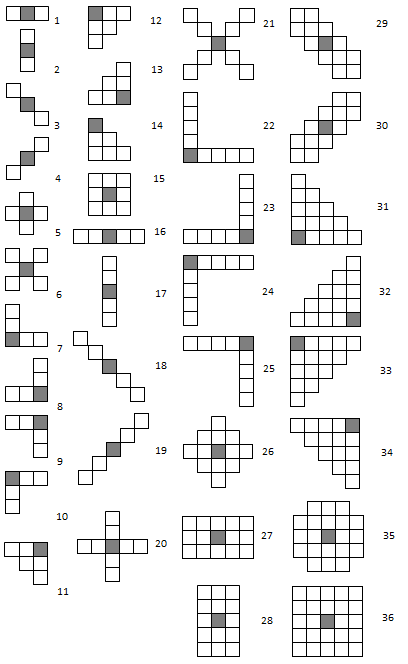
\includegraphics[width=\linewidth]{masks.png}
	\caption{Set of structuring elements (kernels) used for simulations. In grey, structural element's reference point.}
	\label{fig:masks}
\end{figure}

\section{Proposed approach}
\label{sec:method}

In this section we introduce the proposed detector, distinguishing two cases: the detection of morphological filtering on raw images, and the detection in the presence of post-processing (e.g. compression, noise addition, filtering). We will see that the former is a trivial extension of the binary case but has very limited applicability, while the latter requires further attention.

\subsection{Filter Detection on Raw Images}

According to the theory stated in Section \ref{sec:theory}, in the absence of post-processing grayscale morphological operators can be easily and deterministically detected by applying the schema proposed in \cite{de2017detecting} and reported in Figure \ref{fig:scheme}.

\begin{figure*}[!ht]
	\centering
	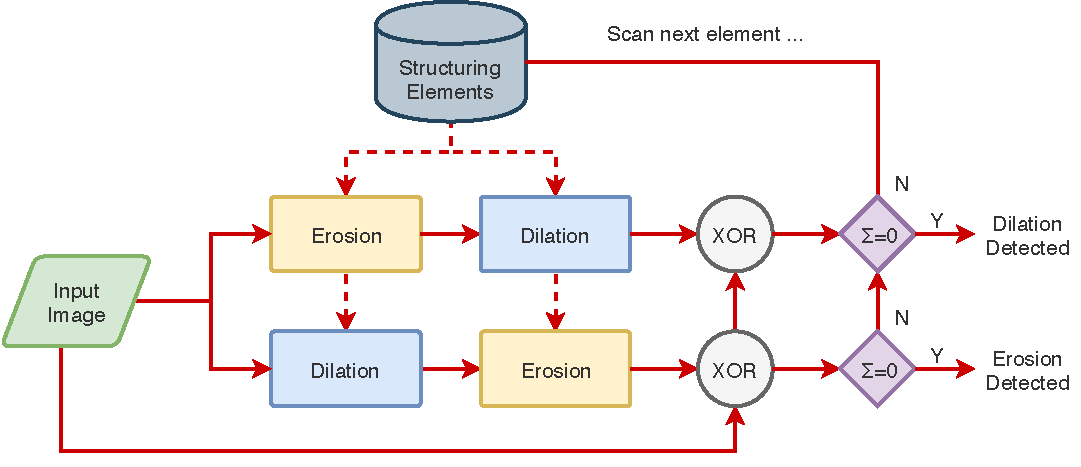
\includegraphics[width=0.7\linewidth]{diagram1}
	\caption{Proposed detection scheme for raw grayscale images.}
	\label{fig:scheme}
\end{figure*}

However, it is worth mentioning that this scenario is rarely verified in grayscale images, which are typically stored in compressed format after filtering. The compression (as well as most other image processing operations) significantly modifies the image, thus hindering the applicability of Theorem~\ref{theorem_1}. As a result, the detector will never report a perfect match between the input eroded (dilated) image and the corresponding opened (closed) version, i.e., it will never output a positive detection.

In the next section we propose an extension of the above algorithm that is able to deal with such scenario. The new algorithm will exploit the traces left by the morphological filters even after post-processing, and will rely on a statistical analysis, thus loosing its deterministic nature. We will see however that it is sufficiently robust to many attacks, and in particular to the JPEG compression.

\subsection{Filter Detection on Post-processed Images}
As mentioned in the previous section, any further processing on the filtered image will modify the pixel values, possibly re-introducing structures that were eliminated by the morphological operator. A further morphological filtering will then produce a non-null effect on the image, which will be revealed by the detector. It is therefore necessary to verify if some traces of the original filter survive the post-processing.

Recalling that the grayscale morphology operates as a local min-max filter, we can expect that it will produce larger variations in the presence of high-contrast structures that match the structural element geometry. On the contrary, unless the post-processing is meant to be extremely visible, it will introduce small gray level variations on the image. Consequently, although we will not have a null difference image at the detector output, we can expect that the local differences will be much smaller for a filtered image than for an original one. An experimental evidence of this fact is provided in Figure \ref{fig:hist_ero}. Here we plot the log-scale histograms of the absolute differences before and after the application of an open operator to a JPEG compressed unfiltered image, and to the relevant JPEG compressed dilated image. Both open and dilation operators have been applied using the kernel mask $35$ in Figure \ref{fig:masks}, and the JPEG quality factor has been set to $QF=95$. It is possible to observe that the histogram referred to the dilated image decreases steeply, with significant bins only for low values of the difference, while the histogram referred to the unfiltered image shows a long tail with significant values also above 50. This means on one side that the compression does not affect the high-contrast structures present in the original image (which are then removed by the following open operator), and on the other side that it does not re-introduce in the filtered image any high-contrast structure sensitive to the filter itself.

\label{subsec:compr_img}
\begin{figure*}[!ht]%
	\centering
	\includegraphics[width=\linewidth]{morphological_example}
	\caption{Histograms of differences before and after application of the open operator to an original image (grayscale version of `r22fa37aft.TIF' from RAISE-1k) and its dilated version. Both images have been JPEG compressed with $QF = 95$. The chart shows the first 50 bins in logarithmic scale. }
	\label{fig:hist_ero}
\end{figure*}

On this basis, we propose to modify the detection scheme as shown in Figure~\ref{fig:scheme_improved}.
\begin{figure*}[!ht]
	\centering
	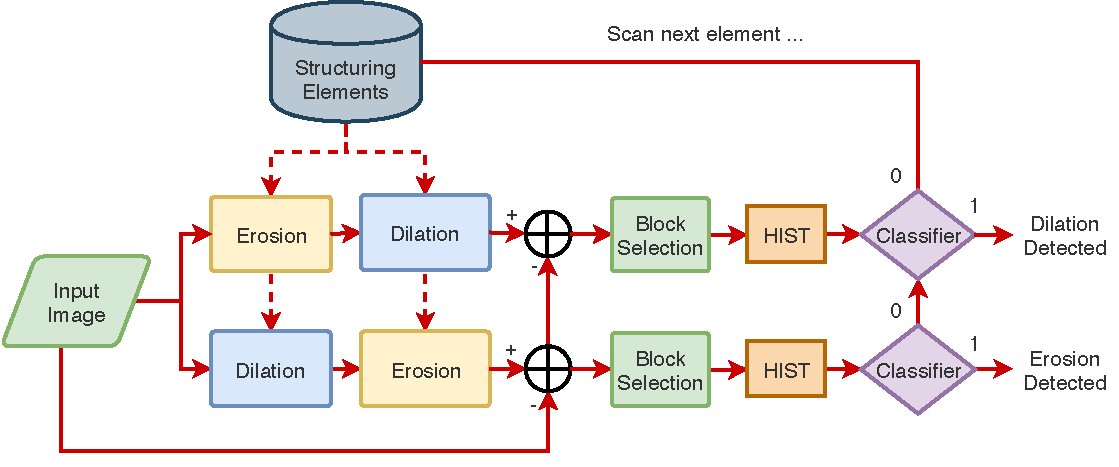
\includegraphics[width=0.7\linewidth]{diagram2}
	\caption{Proposed detection scheme for attacked grayscale images.} 
	\label{fig:scheme_improved}
\end{figure*}
The core of the procedure still involves the application of grayscale opening/closing. In this case, however, we take into consideration the statistical properties of the differences between the input and output images, to see how such residual is distributed. Therefore, we calculate the histogram of the difference image and feed it into a statistical classifier to perform the decision. As far as the classifier is concerned, we adopted a properly trained classifier. %Details on the classifier are provided in the next section.

Finally, we should notice that not all the areas of an image are equally affected by a morphological filter. In particular, the filter has a negligible effect on flat areas, thus possibly jeopardizing the results of the detector. To avoid this problem we decided to limit the analysis to the image regions that contain significant textures or edges. To this purpose, we calculate the block-wise normalized local variance $\alpha$, and we restrict the computation of the histogram to the blocks with $\alpha > \alpha_{th}$, where $\alpha_{th}$ has been empirically set to 0.15. This task is performed by the first processing block in Figure \ref{fig:scheme_improved}. 


\section{Experimental setup}
\label{sec:exp_setup}

In order to assess the performance of the proposed detector, we tested it in various scenarios and we evaluated it in terms of accuracy. In this section we describe such scenarios and the relevant experiments. Furthermore, we introduce the datasets used for the testing, and we provide additional details the relevant training procedure.

\subsection{Datasets}
\label{subsec:datasets}

Three publicly available datasets have been used in the experiments:
\begin{itemize}
	\item The Uncompressed Colour Image Database (UCID) \cite{schaefer2003ucid}, built with the purpose of providing a standard set for performance assessments in image retrieval and compression. The dataset consists of 1,338 uncompressed color images, with fixed sizes of $512\times384$ or $384\times512$ pixels in uncompressed TIFF format.
	\item The Dresden Image Database (DRESDEN) \cite{gloe2010dresden}, originally created for evaluation of forensic techniques related to camera-based information. From their public web-interface, we selected the complete set of RAW images (1,189 uncompressed images, all with fixed size of $3008\times2000$ pixels).
	\item The Raw Images Dataset (RAISE) \cite{dang2015raise}, consisting of 8156 raw images with resolutions ranging from $3,008\times2,000$ to $4,928\times3,264$ pixels. Authors provide also smaller subsets, among which we selected the one containing 1,000 images (RAISE-1k).
\end{itemize}

The three datasets were selected to diversify the range of resolutions in the experimental tests. In order to evaluate our proposed schema, all the images were converted to grayscale with a depth of 8 bits.

\subsection{Testing scenarios}
\label{subsec:test_scenarios}
The proposed detector has been tested in various practical scenarios:%. It is to be pointed out that we did not consider the case of unattacked images, which is by definition deterministic, as previously discussed, and provides therefore 100\% accuracy.

\begin{itemize}
	\item The first set of tests were performed in order to understand the impact of the parameters as well as to select a proper classifier. Based on the setups found on this set of tests, we kept the best setups (in terms of performance) for the next tests.
	
	\item The second set of tests refers to the detection of morphological filtering. In this case, we want to establish the accuracy of the detector in discriminating filtered vs. pristine (unfiltered) images, in classifying the type of operator (erosion vs. dilation), and finally in determining the exact structuring element used for filtering, both in uncompressed and JPEG compressed images with various quality factors. 
	
	\item The third set of tests concerns robustness against noise. The test image is contaminated with random noise and then compressed, and we evaluate the accuracy of the detector in determining the presence and type of filtering and the structuring element used.
	
	\item Finally, we want to determine the capability of our approach in distinguishing between morphological filters and other filters that produce similar results. In particular, we considered Gaussian lowpass and median filtering. In both cases, the filtered images are compressed and passed to the detector to reveal possible false alarms.
	
\end{itemize}

It is worth noting that, due to the properties analysed in Section~\ref{sec:theory}, in the presence of a cascade of different basic operators (erosion and dilation), the detector will reveal the last operator applied. Accordingly, when processing an opened or a closed image, the detector will reveal the last dilation or erosion, respectively. Furthermore, in the presence of a cascade of the same basic operator, the detector will reveal a single erosion or dilation with the composed structuring element. Therefore, in the experimental section we will just consider erosion and dilation detection, even if the image may have been potentially processed with more complex combinations of filters.


\section{Experimental Results and Discussion}
\label{sec:experiments}

In this section, all experimental tests carried out are described. %In subsection IV-A, the selected datasets and the processing of their content are presented, together with results related to uncompressed data; while subsection IV-B is dedicated to the analysis of compressed data. 
All  tests are performed using Python 3.6 and libSVM on a standard machine (Macbook Pro 2016 2,3GHz 4-kernel Intel Core i5, 8GB ram).

\subsection{The Sensibility and the Choice of the Classifiers}
\label{subsec:sensibity}

In order to understand the impact of the parameters as well as to select a proper classifier, we ran some experiments on a subset of images. After that, we empirically determined the values for these parameters. Table~\ref{tab:sensibility} summarizes these parameters, their meaning and how their values were decided.

\begin{table*}[t!]
	\centering
	\caption{Parameters selection.}
	\label{tab:sensibility}
	\resizebox{\linewidth}{!}{
		\begin{tabular}{p{3cm}|p{5cm}|p{4cm}|p{5cm}}
			\hline\hline
			\textbf{Parameter/ Classifier} & \textbf{Meaning} & \textbf{Range} &  \textbf{Empirical Value/Selection} \\
			\hline
			Image resolution & The size of the analyzed region of interest & $384 \times 512$  to $4928 \times 3264$& Good results for resolution higher than $1000 \times 1000$.\\
			\hline
			Block Selection Threshold $\alpha_{th}$ and Block Size $s$ & Erosion and dilation have a negligible effect on flat areas, thus these two parameters allow the method to effectively work on non-flat blocks only. & $\alpha_{th} \ge 0$, $\alpha = 0$ means all pixels in the block has the same values.
			
			$ s \in \{3 \times 3, 5 \times 5, ...\}$ & $ \alpha_{th} = 0.15$ and $s = 3 \times 3$.\\
			\hline
			$n$ & Number of bins of the analyzed histograms.& $0 \le n \le 256$ & Even if for $n > 30$ we already achieve 90\% accuracy, we set $n$ at the highest value, i.e., considering all bins.\\
			\hline
			The classifiers & & SVM, KNN, Linear Regression, and others & SVM with RBF kernel and grid search provides the best performance. \\							
			\hline\hline
	\end{tabular}}
\end{table*}

The classifier receives in input the histogram of the differences between the input image and the relevant opened (closed) image and returns a binary decision. An important aspect is the training of the classifier. In fact, there is a clear dependency of the image statistics on the level of compression applied, which is reflected on the characteristics of the histogram. As an example, Figure \ref{fig:hist_ero_80} shows the same situation of Figure \ref{fig:hist_ero} at a lower quality factor. It can be observed that the two distributions are still well separable, but the histogram related to the filtered image shows a longer tail, due to the larger artifacts introduced by the compression.

\begin{figure}[t!]%
	\centering
	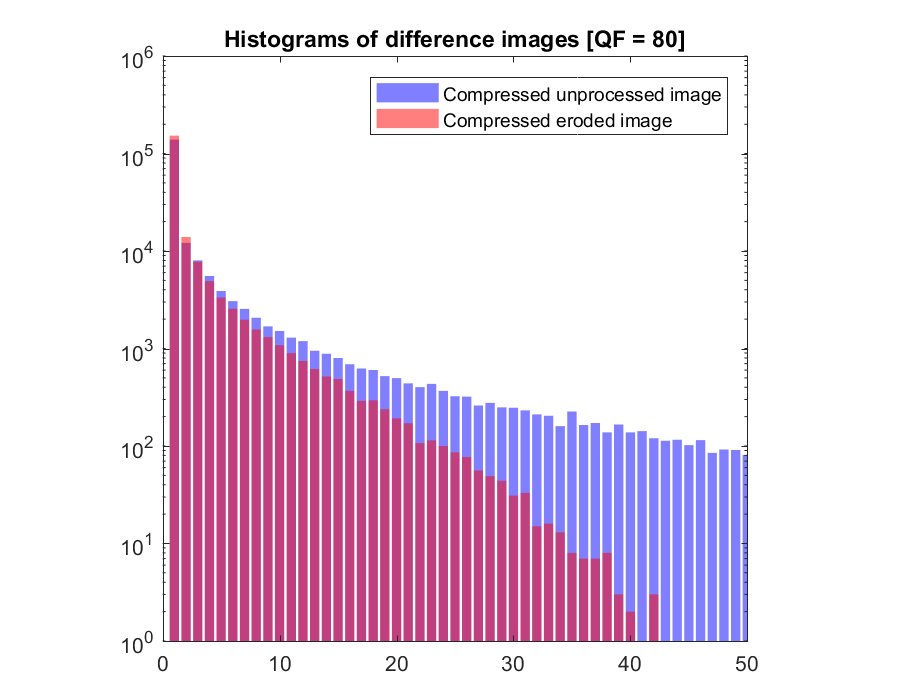
\includegraphics[width=\linewidth]{hist_ero_80.eps}
	\caption{Same case of Fig. \ref{fig:hist_ero} after compression at $QF = 80$.}
	\label{fig:hist_ero_80}%
\end{figure}

\begin{figure}[t!]
	\centering
	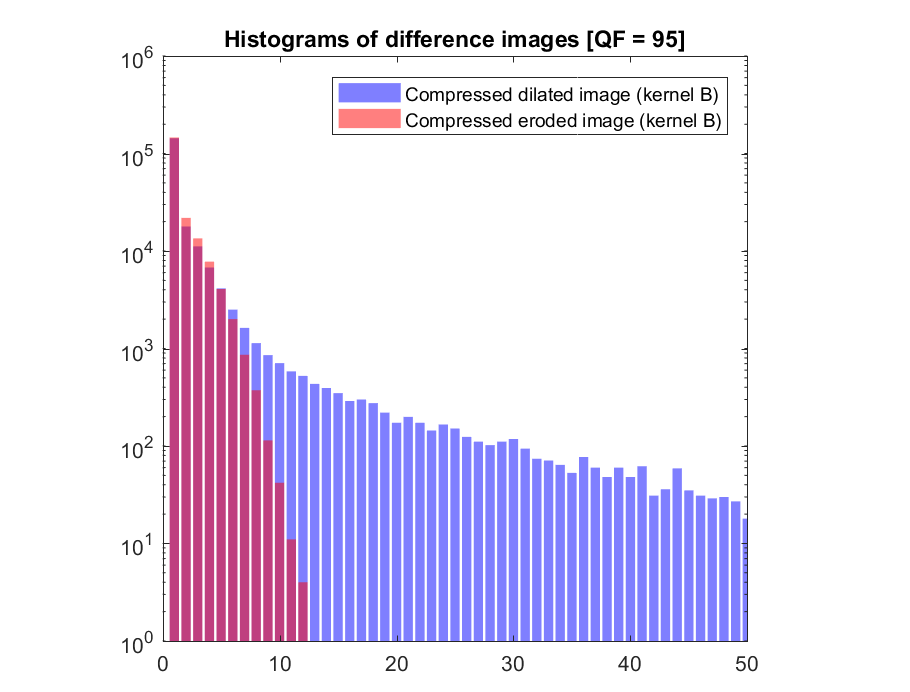
\includegraphics[width=\linewidth]{hist_dil_ero_same.eps}
	\caption{Histograms resulting from dilated and eroded images produced with the same structuring element, after compression at QF=95 and erosion detection. \textbf{Figure 9: since you decided to go for K instead of B maybe is better to cite K and K*?}}
	\label{fig:hist_dil_ero_same}
\end{figure}

\begin{figure}[t!]
	\centering
	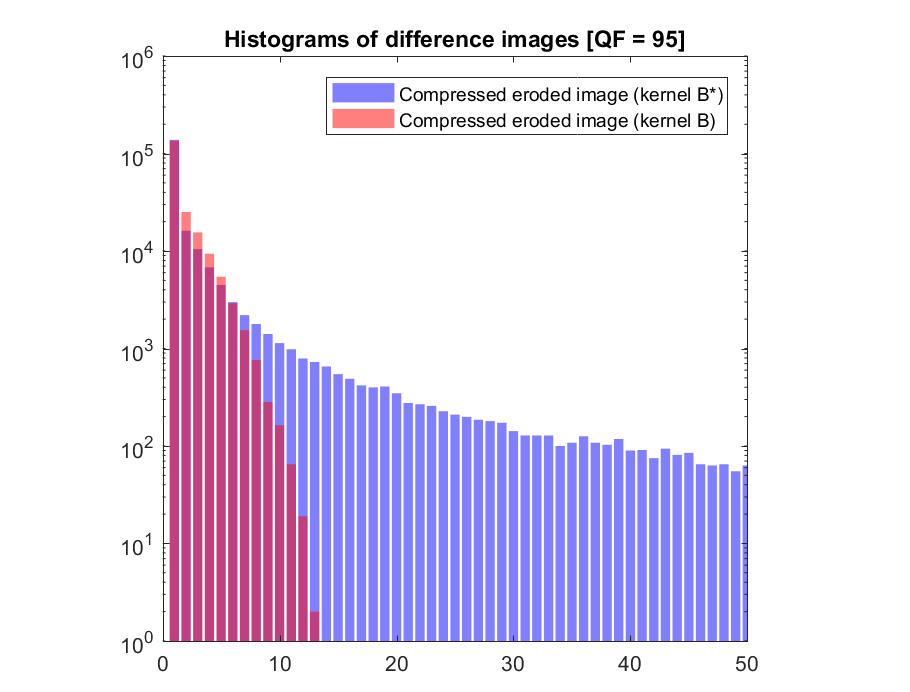
\includegraphics[width=\linewidth]{hist_ero_ero_diff.eps}
	\caption{Histograms resulting from eroded images produced with unrelated structuring elements, after compression at QF=95 and erosion detection.\textbf{Figure 9: since you decided to go for K instead of B maybe is better to cite K and K*?}}
	\label{fig:hist_ero_ero_diff}
\end{figure}

\begin{figure}[t!]
	\centering
	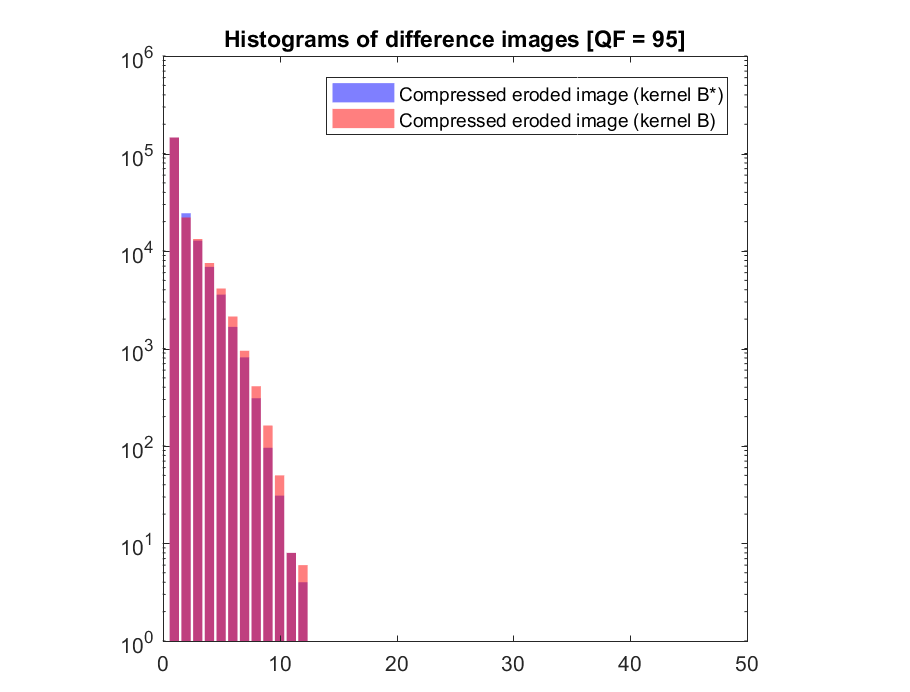
\includegraphics[width=\linewidth]{hist_ero_ero_albero.eps}
	\caption{Histograms resulting from eroded images produced with structuring element $B$ and its dilated version $B^*$, after compression at QF=95 and erosion detection.\textbf{Figure 9: since you decided to go for K instead of B maybe is better to cite K and K*?}}
	\label{fig:hist_ero_ero_albero}
\end{figure}

Accordingly, we decided to train a set of classifiers for varying JPEG quality factors, from 100 to 70. During the test phase, we tested with different classifiers: k-NN, decision trees, naive Bayes classifier, and SVM, and empirically decided to use SVM with the radial basis function (RBF) kernel. 

We also note that given the appropriate quality factor, the histograms of differences show a peculiar behavior only if the detector parameters match the input filter in both the operator (erosion or dilation) and the structural element (kernel), whereas such behavior is never found in all the other combinations. It is important to notice that the application of the detector to an unfiltered image or to an image filtered with a different combination of operator and/or kernel produces similar results, i.e., only the matching detector responds to the filtered image. As an example, in Figure \ref{fig:hist_dil_ero_same} we show the histograms deriving from the application of an erosion detector to an eroded and a dilated image, both with the same kernel. It can be observed that the dilated image responds similarly to the uncompressed image in Figure \ref{fig:hist_ero}. Analogously, in Figure \ref{fig:hist_ero_ero_diff}, we compare the histograms deriving from the erosion detector applied to two eroded images, one with the same kernel and the other with a different one. Also in this case, the image filtered with a different kernel responds as unfiltered. Finally, in Figure \ref{fig:hist_ero_ero_albero} we show the case of application of the erosion detector to two images filtered with kernels belonging to the same group (i.e., one can be obtained from the other by dilation). As expected from Theorem~\ref{theorem_2}, the two histograms are almost overlapped, since both show the statistical properties of a filtered image.

For some other choices, for example the block size or $\alpha_{th}$, all values are empirically selected and are reported in Table~\ref{tab:sensibility}. 

\subsection{Distinguishing between Pristine versus Morphological Filtered Images}
\label{sec:compr_res}

\subsubsection{Experimental Results on Raw Images}

We ran a test on uncompressed images in order to confirm the deterministic nature of the proposed approach on unpressed images. Since the detection strategy in this case is the very same proposed in \cite{de2017detecting}, we followed their general approach for deriving results relative to raw grayscale images. Each image has been processed with erosion and dilation operators considering all the 36 kernels.
All images, along with their unprocessed versions, were fed to both dilation and erosion detectors. For each image, all 36 kernels are tested, returning either the largest kernel with perfect match between input and output or no detection if all kernels fail. All three datasets result in 100\% accuracy in discriminating the presence and the type of morphological filter, as reported in Table \ref{tab1:det_acc}.

\begin{table}[!ht]
	\centering
	\caption{Detection accuracy for all three datasets for uncompressed images.}
	\label{tab1:det_acc}
	\begin{tabular}{|l|l|l}
		\hline\hline%\cline{2-3}
		\multicolumn{1}{c|}{}		     & \multicolumn{2}{c}{\textbf{Detector}}	           				    \\ 
		\cline{2-3}
		\multicolumn{1}{c|}{\textbf{Filter}}    & \multicolumn{1}{c|}{erosion} & \multicolumn{1}{c}{dilation} \\ 
		\hline%\hline
		\multicolumn{1}{c|}{no filter} & \multicolumn{1}{c|}{0\%} 	& \multicolumn{1}{c}{0\%}      \\ \hline
		\multicolumn{1}{c|}{erosion}   & \multicolumn{1}{c|}{100\%}   & \multicolumn{1}{c}{0\%}      \\ \hline
		\multicolumn{1}{c|}{dilation}  & \multicolumn{1}{c|}{0\%}     & \multicolumn{1}{c}{100\%}    \\ 
		\hline\hline
	\end{tabular}
\end{table}

\begin{sidewaystable*}[]
	\centering
	\caption{Confusion matrix on erosion detection for multiple kernels. Dataset: Raise, QF = 90, full resolution. Values are normalized and are in percentage.}
	\label{table:confusion}
	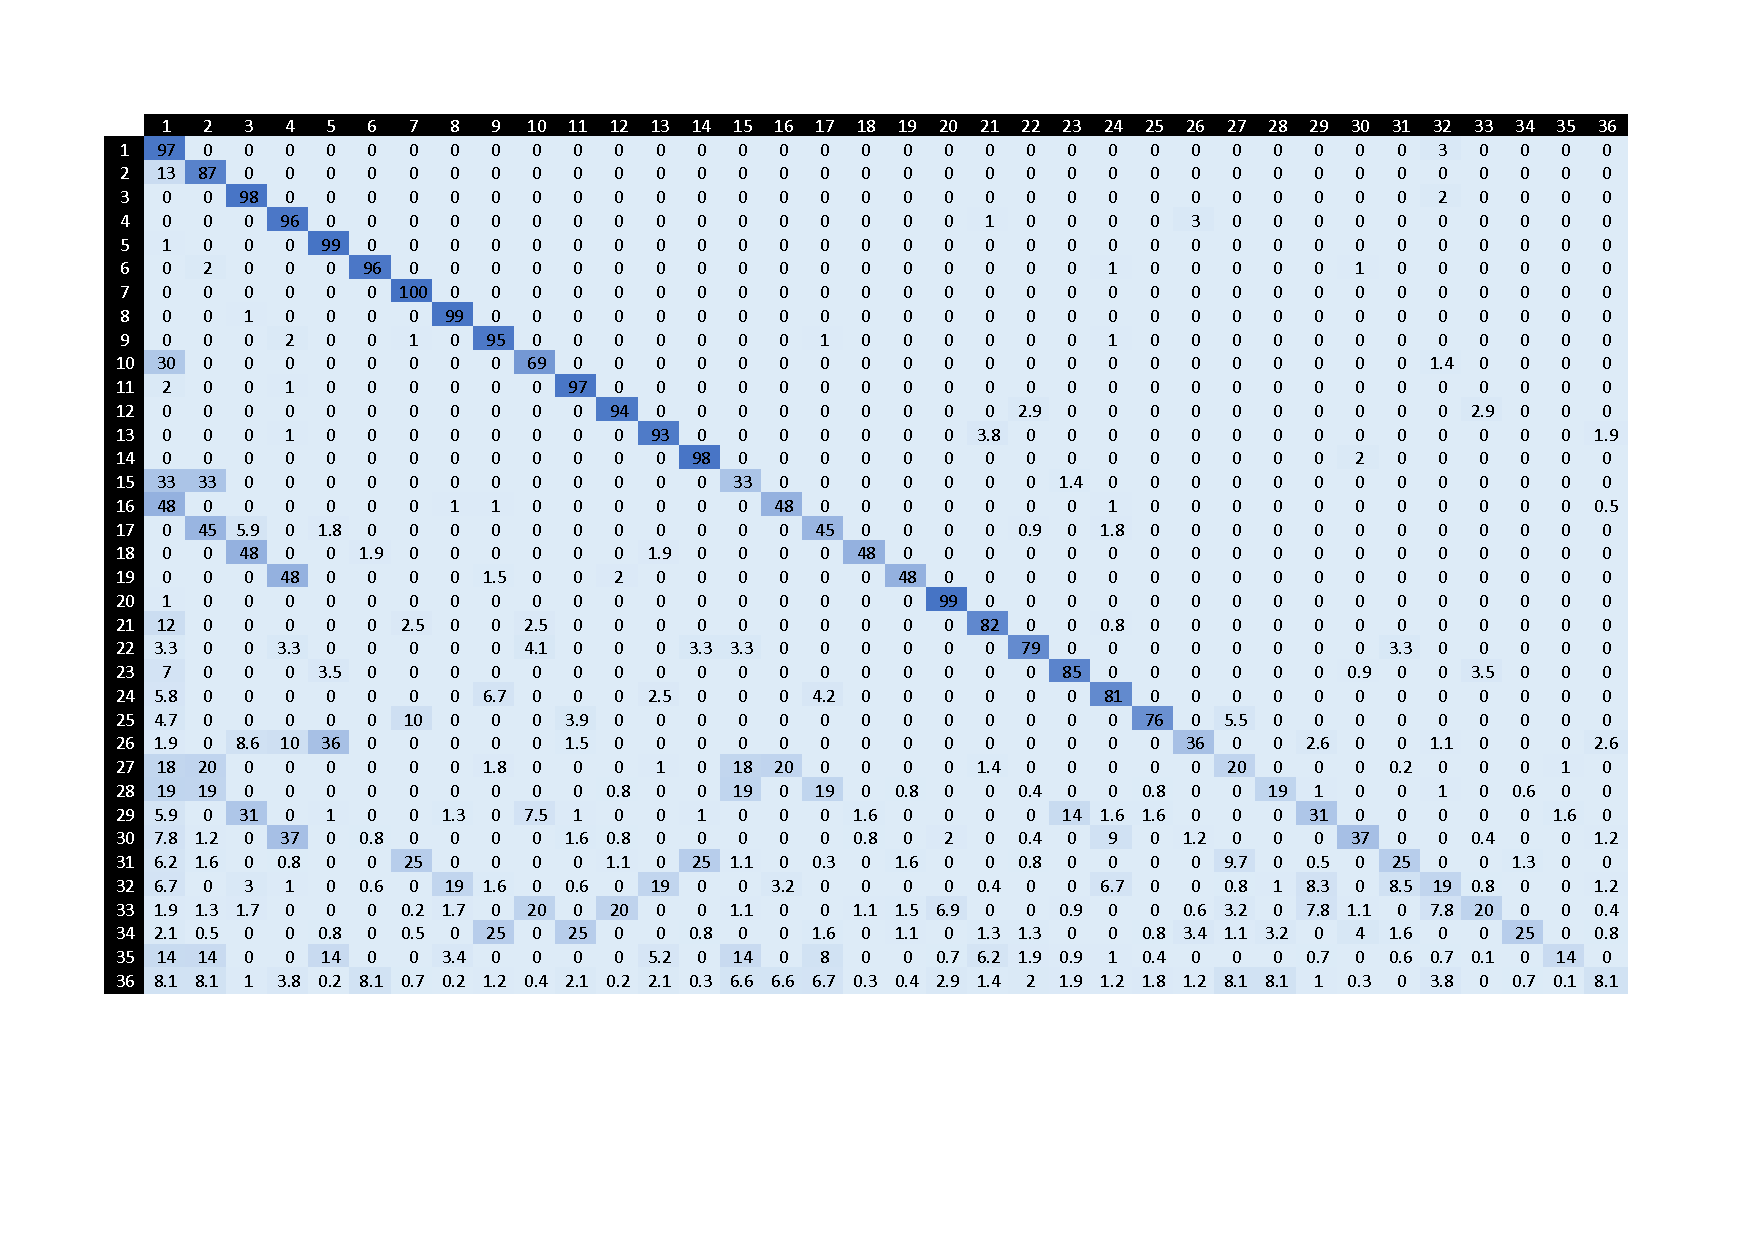
\includegraphics[width=\linewidth]{confusion}
\end{sidewaystable*}

\subsubsection{Experimental Results on JPEG Compressed Images}
%
In order to test the approach on JPEG compressed images, we considered a set of seven different quality factors with $QF \in \{100,95,90,85,80,75,70\}$, with 14 $(7\times 2)$ binary classifiers, respectively,
using a Gaussian kernel with grid-search for the parameters. We apply k-Fold validation with $k = 10$. Shown in Table~\ref{table:detection_results} are the average results (over all kernels) of the proposed method on three datasets at the seven quality factors. The detailed results for all kernels, both two morphological operators over all three datasets are reported in Tables~\ref{table:uciderosion} - \ref{table:raisedilation} in \ref{app:detailed_compress}. According to the results, we can observe that the proposed method can provide high detection performance on low compression level (i.e., high factor quality with $QF \ge 80$) with accuracy equal or above $76.8\%$ on all datasets. At higher compression level, the performance reduces significantly. The resolution also plays an important role as it can be grasped from the results. Indeed, UCID has lower performance with respect to Dresden and Raise. It is also interesting to notice that there is little difference between Dresden and Raise. To have a deeper understanding of the impact of the image resolution, we ran another test on different image resolutions: the proposed method achieves good performance (over 90\%) for resolution from about $1,000 \times 1,000$. Shown in Figure~\ref{fig:resolutions} are results over 36 kernels on erosion detection forr RAISE-1k images.%Table~\ref{table:resolutionerosion} in \ref{app:detailed_compress}. 

\begin{figure}[h!]
	\centering
	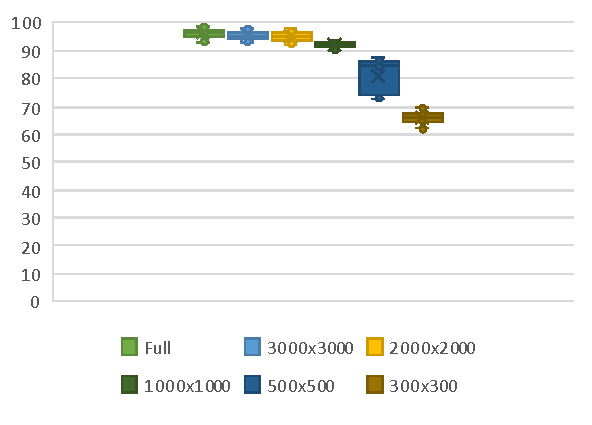
\includegraphics[width=\linewidth]{resolutions.pdf}
	\caption{Results (computed as percentage) on erosion detection under different resolutions. Dataset: Raise, QF = 90. All 36 kernels are computed and their results are shown in the error bars.}
	\label{fig:resolutions}
\end{figure}

\begin{table*}[t!]
	\centering
	\caption{Morphological filtering detection results on all three datasets  using SVM with RBF kernel, 10-fold cross validation. The numbers are in percentage and each of them is the average performance (for distinguishing between pristine versus filtered images) over all 36 kernels. Detailed results are reported in Tables~\ref{table:uciderosion} - \ref{table:raisedilation}.}
	\label{table:detection_results}
	%\resizebox{\linewidth}{!}{
		\begin{tabular}{l|l|ccccccc}
			\hline\hline
			\textbf{Dataset} & \textbf{Operator} & \textbf{QF = 100} & \textbf{95} & \textbf{90} & \textbf{85} & \textbf{80} & \textbf{75} & \textbf{70} \\
			\hline
			\textbf{UCID} & Erosion & 100 & 90.86 & 82.62 & 79.63 & 77.45 & 67.41 & 64.42 \\
			& Dilation & 100 & 90.16 & 82.86 & 79.95 & 76.80 & 68.77 & 64.94 \\
			\hline
			\textbf{Dresden} & Erosion & 100 & 97.56 & 96.94 & 95.20 & 88.73 & 79.85 & 78.34 \\
			& Dilation & 100 & 97.93 & 96.82 & 96.11 & 88.74 & 81.08 & 75.08 \\
			\hline
			\textbf{Raise} & Erosion & 100 & 98.66 & 96.25 & 94.82 & 89.00 & 80.42 & 78.55 \\
			& Dilation & 100 & 97.98 & 97.43 & 93.72 & 91.02 & 80.49 & 78.53 \\
			\hline\hline
	\end{tabular}%}
\end{table*}

\subsection{Detector Robustness Analysis}
\label{subsec:result_attacks}

The second test in this set is to analyse the impact of different kernels. We applied all kernels and then tried to detect them using different classifiers. Shown in Table~\ref{table:confusion} is the confusion matrix of the erosion detection (similar results were obtained on dilation detection). According to the results, the detector was able to recognize small size kernels (kernels from 1 to 14, please see again Figure~\ref{fig:masks} for the kernels), or larger kernels in special shape (kernels 20 to 25), but poorly classified the others. This is understandable as a consequence of Theorem~\ref{theorem_2}.

The third set of tests concerns analysis of robustness against noise addition. In the first test, morphological filtering is applied to each image and then this is contaminated with a noise. Five different attacks - pepper \& salt noise, Gaussian filtering, median filtering, scaling at 1.1x and scaling at 0.9x - were applied and average results (on all kernels) for dilation detection on RAISE1k are correspondingly: 97.92\%, 81.21\%, 87.94\%, 67.44\%, and 67.81\% (the results are summarized in Figure~\ref{fig:attacks_1}. According to the results, we can claim that the proposed method is robust against noise addition but not against processing involving interpolation (e.g., resizing). 

\begin{figure}[h!]
	\centering
	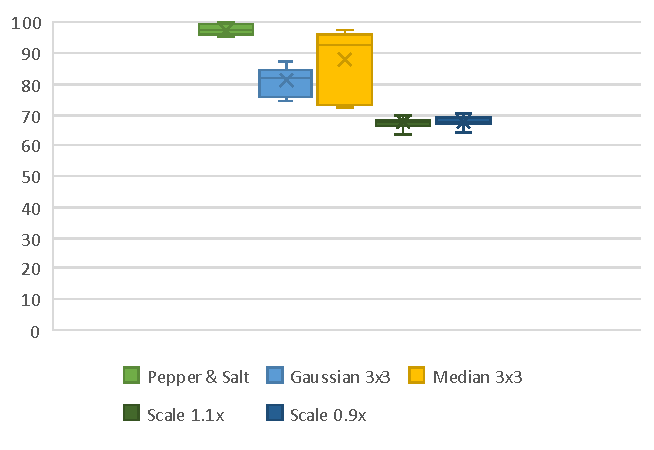
\includegraphics[width=\linewidth]{attacks_1.pdf}
	\caption{Results (computed as percentage) on dilation detection under different attacks. Dataset: RAISE-1k, full resolution, QF = 100, using SVM with RBF kernel, 10-fold cross validation. All 36 kernels are computed and the results are shown in the error bars.}
	\label{fig:attacks_1}
\end{figure}

We applied a further test to understand if the proposed method can still detect the morphological filter after two level of processing where the second one is a compression. Thus, each image after a morphological filter is first contaminated with a noise, and then is compressed under different quality factors.  The results in Table~\ref{table:attacks2} show that the proposed method can still detect the morphological filter, however, its performance is getting worst as the compression level increases.  

\begin{table}[t!]
	\centering
	\caption{Results on erosion detection on Raise under different attacks, using SVM with RBF kernel, 10-fold cross validation.}
	\label{table:attacks2}
	\begin{tabular}{c|ccc}
		\hline\hline
		\textbf{QF} & \textbf{Pepper \& Salt}&\textbf{Gaussian (3x3)}&\textbf{Median Filter (3x3)}\\
		\hline
		100&97.92&81.21&87.94\\
		95&95.72&81.14&86.44\\
		90&95.19&81.01&84.27\\
		85&91.79&79.16&80.67\\
		80&86.99&78.76&80.57\\
		75&83.04&75.06&76.42\\
		70&81.23&70.24&71.49\\
		\hline\hline	
	\end{tabular}
\end{table}

\subsection{Morphological Filters versus Other Filters }
\label{subsec:results_different_filters}

Finally, we want to determine the capability of our approach in distinguishing between morphological filters from other filters that produce similar results. In particular, we considered three filters: pepper \& salt, Gaussian lowpass and median filtering. In all cases, the filtered images are uncompressed and passed to the detector to reveal possible false alarms. 
In this experiment, we trained the erosion versus pristine classifier with 800 uncompressed images from RAISE in full resolution. The trained classifier is then applied to the rest of the 200 images, filtered with pepper \& salt, Gaussian lowpass and median filters. We got the average number of false positives (over 200 images) for pepper \& salt, Gaussian $3 \times 3$, Gaussian $5 \times 5$, median filter $3 \times 3$, and median filter $5 \times 5$ are 3.51\%, 5.72\%, 5.28\%, 14.11\%, and 13.17\%, respectively. The results are summarized in Figure~\ref{fig:different_filters}.  
This confirms that the proposed method can distinguish between morphological filter from other filters. Only in the case of median filters the confusion increases, but this is very reasonable, since in the case of grayscale images the effect of morphological filters and median filters are very similar.

\begin{figure}[h!]
	\centering
	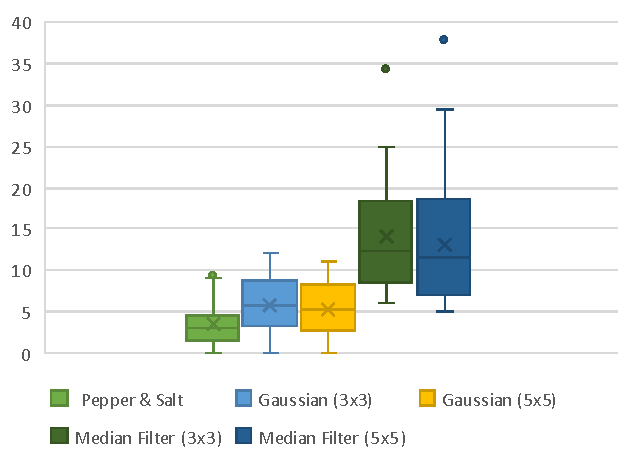
\includegraphics[width=\linewidth]{different_filters.pdf}
	\caption{False Positive (computed as percentage) on 200 images from RAISE on erosion detection over all 36 filters. Images are in raw format, full resolution. The classifiers were trained on 800 images (eroded vs. non-filtered) and tested on the rest 200 images (filtered with pepper \& salt, Gaussian and median).\textbf{Can we scale it 0-100 as previous one so it is evident we do not have huge errors?}}
	\label{fig:different_filters}
\end{figure}


\section{Conclusions}
\label{sec:conclusions}
In this work we propose an effective detection strategy to assess the use of morphological filtering in a grayscale context. We deal with uncompressed images proposing a deterministic approach, reflection of the binary domain scenario, based on mathematical properties enjoyed by basic morphological operators. We additionally propose a modified pipeline to detect morphological processing in compressed images, exploiting difference histogram information as feature for  classification. Finally, we present a testing phase in which both uncompressed and compressed scenarios are taken into consideration. Results show the effectiveness of our proposed approach in both cases.  

\bibliography{refs}
\bibliographystyle{IEEEtran}

\begin{comment}
\newpage
\appendix
\setcounter{table}{0}

\section{Detailed Results}
\label{app:detailed_compress}

\begin{table*}[ht!]
	\centering
	\begin{minipage}{0.48\linewidth}
		\centering
		\caption{Results on erosion detection on UCID using SVM with RBF kernel, 10-fold cross validation.}
		\label{table:uciderosion}
		\resizebox{\linewidth}{!}{
			\begin{tabular}{c|ccccccc}
				\hline\hline
				\textbf{K}&\textbf{QF = 100}&\textbf{95}&\textbf{90}&\textbf{85}&\textbf{80}&\textbf{75}&\textbf{70}\\
				\hline
				1&100&90.42&83.42&79.06&75.83&64.25&63.34\\
				2&100&90.89&82.73&79.7&76.23&65.2&64.23\\
				3&100&90.34&82.57&80.69&77.19&66.06&64.91\\
				4&100&89.61&83.06&80.74&76.99&65.31&63.92\\
				5&100&90.15&83.14&80.91&77.62&65.09&62.95\\
				6&100&90.56&82.49&81.42&78.42&65.55&63.56\\
				7&100&91.2&82.67&81.03&78.66&66.22&64.53\\
				8&100&92.2&82.62&80.17&78.19&65.24&65.45\\
				9&100&92.69&83.59&80&79.1&65.9&64.87\\
				10&100&92.89&84.08&80.65&79.67&65.78&64.5\\
				11&100&93.09&83.41&79.88&80.26&65.59&65.28\\
				12&100&93.48&83.63&80.87&80.08&64.86&65.41\\
				13&100&94.47&83.62&80.73&79.93&64.35&64.61\\
				14&100&93.59&84.32&80.25&79.59&64.49&65.6\\
				15&100&94.4&84.02&79.3&80.32&65.07&64.72\\
				16&100&88.41&82.22&80.45&76.24&69.13&62.8\\
				17&100&88.49&83.18&81.17&76.4&69.07&63.66\\
				18&100&88.78&83.72&81.99&76.76&69.08&63.69\\
				19&100&89.09&83.29&82.21&76.7&68.8&63.53\\
				20&100&89.07&83.67&82.96&77.01&69.23&64.52\\
				21&100&88.87&83.86&83.18&76.62&69.86&64.71\\
				22&100&89.13&84.17&83.86&76.12&69.63&65.69\\
				23&100&89.99&84.82&83.4&76.52&70.3&65.67\\
				24&100&90.35&84.95&83.55&77.34&70.59&65.73\\
				25&100&90.19&84.52&84.19&78.11&70.92&65.93\\
				26&100&89.87&80.42&74.24&75.44&68.14&62.58\\
				27&100&90.83&81.14&74.92&75.64&68.08&62.74\\
				28&100&90.44&81.34&75.37&75.18&67.81&62.5\\
				29&100&90.33&80.88&76.1&75.88&68.61&62.69\\
				30&100&89.98&80.55&75.74&75.71&68.24&62.64\\
				31&100&90.61&80.2&75.41&76.34&67.99&63.05\\
				32&100&90.67&80.56&76.02&76.72&68.44&63.03\\
				33&100&91.31&80.39&75.64&77.12&68&63.58\\
				34&100&91.03&80.48&76.41&77.92&68.24&63.61\\
				35&100&91.34&80.29&77.04&77.78&68.29&64.04\\
				36&100&92.26&80.36&77.5&78.46&69.2&64.03\\
				\hline
				\textbf{Avg.}&\textbf{100}&\textbf{90.86}&\textbf{82.62}&\textbf{79.63}&\textbf{77.45}&\textbf{67.41}&\textbf{64.12}\\
				\hline\hline	
		\end{tabular}}
	\end{minipage}
	\begin{minipage}{0.48\linewidth}
		\centering
		\caption{Results on dilation detection on UCID using SVM with RBF kernel, 10-fold cross validation.}
		\label{table:uciddilation}
		\resizebox{\linewidth}{!}{
			\begin{tabular}{c|ccccccc}
				\hline\hline
				\textbf{K}&\textbf{QF = 100}&\textbf{95}&\textbf{90}&\textbf{85}&\textbf{80}&\textbf{75}&\textbf{70}\\
				\hline
				1&100&89.24&83.18&80.05&75.29&65.35&63.34\\
				2&100&88.4&82.29&81.01&76.16&65.08&63.93\\
				3&100&88.1&81.66&81.54&75.77&65.49&64.77\\
				4&100&88.11&82.34&81.51&75.33&65.17&65.4\\
				5&100&89.09&82.67&82.35&74.89&65.95&66.36\\
				6&100&89.99&82.85&82.43&75.42&65.94&67.35\\
				7&100&89.28&82.35&83.15&75.81&65.53&67.89\\
				8&100&89.9&83.04&82.9&75.06&66.12&68.67\\
				9&100&90.46&83.42&82.3&75.99&66.64&67.95\\
				10&100&91.03&82.55&81.76&75&67.59&68.91\\
				11&100&90.76&83.13&80.9&75&67.69&68.3\\
				12&100&91.28&83.21&81.69&75.84&67.9&67.33\\
				13&100&91.44&83.85&81.01&76.02&68.6&66.94\\
				14&100&90.49&83.33&81.7&76.56&68.58&66.35\\
				15&100&91.33&84.22&82.61&75.65&69.13&66.05\\
				16&100&90.05&82.22&81.15&77.25&70.23&62.8\\
				17&100&90.66&82.24&81.36&77.96&70.63&62.47\\
				18&100&90.5&82.21&81.39&78.31&70.22&63.29\\
				19&100&90.14&82.77&81.87&78.69&70.71&63.16\\
				20&100&89.72&83.18&81.64&78.59&70.46&63.26\\
				21&100&89.68&83.39&81.82&78.39&70.2&63.25\\
				22&100&89.94&83.58&82.17&78.19&70.05&63.96\\
				23&100&90.06&83.57&82.45&77.88&69.65&64.52\\
				24&100&89.97&83.96&83.34&78.36&70.41&64.91\\
				25&100&90.89&84.61&83.67&77.88&70.18&64.91\\
				26&100&89.91&81&73.87&75.78&69.02&62.27\\
				27&100&89.73&80.83&74.19&76.59&69.83&63.22\\
				28&100&89.99&80.75&74.78&76.2&70.08&63.66\\
				29&100&89.58&81.46&75&76.21&70.63&63.38\\
				30&100&89.76&82.18&74.7&76.52&70.24&63.19\\
				31&100&90.08&82.47&75.24&76.92&70.01&63.77\\
				32&100&90.73&82.92&76.12&77.72&69.69&63.46\\
				33&100&90.41&82.88&75.96&78.03&69.94&64.2\\
				34&100&91.27&83.3&76.42&78.67&70.55&64.98\\
				35&100&91.62&84.22&77.26&78.44&70.67&64.63\\
				36&100&92.09&85.22&76.96&78.57&71.66&65.01\\
				\hline
				\textbf{Avg.}&\textbf{100}&\textbf{90.16}&\textbf{82.86}&\textbf{79.95}&\textbf{76.80}&\textbf{68.77}&\textbf{64.94}\\
				\hline\hline	
		\end{tabular}}
	\end{minipage}
\end{table*}

\begin{table*}[ht!]
	\centering
	\begin{minipage}{0.48\linewidth}
		\centering
		\caption{Results on erosion detection on Dresden using SVM with RBF kernel, 10-fold cross validation.}
		\label{table:dresdenerosion}
		\resizebox{\linewidth}{!}{
			\begin{tabular}{c|ccccccc}
				\hline\hline
				\textbf{K}&\textbf{QF = 100}&\textbf{95}&\textbf{90}&\textbf{85}&\textbf{80}&\textbf{75}&\textbf{70}\\
				\hline
				1&100&99.03&98.85&97.01&87.43&78.63&76.19\\
				2&100&99.04&97.91&97.24&88.17&78.3&76.7\\
				3&100&98.32&97.83&97.67&89.16&78.64&76.22\\
				4&100&97.41&97.41&97.41&88.31&79.59&76.2\\
				5&100&97.12&96.92&96.75&88.29&78.84&76.3\\
				6&100&97.74&97.28&95.78&87.49&79.73&76.66\\
				7&100&98.66&97.74&95.15&87.41&79.33&77.39\\
				8&100&98.18&97.22&94.63&87.22&78.57&77.18\\
				9&100&97.72&96.58&94.76&87.66&79.42&76.73\\
				10&100&96.76&96.45&93.76&87.88&78.93&77.3\\
				11&100&95.9&95.9&94.61&88.45&78.02&78.02\\
				12&100&96.28&95.93&95.17&88.11&78.05&77.9\\
				13&100&96.15&96.15&94.33&87.41&78.76&78.35\\
				14&100&97&96.73&95.24&86.53&78.35&78.35\\
				15&100&96.34&96.34&95.8&86.72&79.28&79.02\\
				16&100&98.95&97.93&96.52&89.32&80.03&82.23\\
				17&100&98.2&97.8&97.01&89.85&79.32&81.79\\
				18&100&97.58&96.91&96.81&90.15&79.56&82.78\\
				19&100&97.84&97.59&96.51&90.05&79.4&83.08\\
				20&100&98.17&98.17&97.21&89.45&80.18&83.64\\
				21&100&98.73&97.78&96.96&89.25&79.99&83.46\\
				22&100&98.09&97.98&96.56&88.97&79.43&84.22\\
				23&100&98.17&97.66&95.69&88.55&79.61&84.65\\
				24&100&98.03&96.72&95.69&89&78.99&84.18\\
				25&100&97.07&97.07&95.62&88.3&78.83&84.58\\
				26&100&98.03&96.65&93.89&89.3&81.44&73.26\\
				27&100&97.22&95.72&94.15&88.9&82.37&73.62\\
				28&100&97.95&96.57&94.19&89.56&82.33&73.98\\
				29&100&97.84&96.58&93.67&89.71&81.64&74.6\\
				30&100&98.19&96.44&94.08&90.29&81.11&75.4\\
				31&100&97.97&96.06&93.95&90.16&81.26&75.12\\
				32&100&97.16&96.71&93.5&89.64&81.41&75.53\\
				33&100&96.67&96.27&93.16&88.65&80.83&75.87\\
				34&100&96.15&96.15&92.9&89.32&81.14&76.29\\
				35&100&96.68&96.25&92.03&89.67&81.31&76.6\\
				36&100&95.76&95.69&91.64&89.83&81.89&76.76\\
				\hline
				\textbf{Avg.}&100&\textbf{97.56}&\textbf{96.94}&\textbf{95.20}&\textbf{88.73}&\textbf{79.85}&\textbf{78.34}\\
				\hline\hline	
		\end{tabular}}
	\end{minipage}
	\begin{minipage}{0.48\linewidth}
		\centering
		\caption{Results on dilation detection on Dresden using SVM with RBF kernel, 10-fold cross validation.}
		\label{table:dresdendilation}
		\resizebox{\linewidth}{!}{
			\begin{tabular}{c|ccccccc}
				\hline\hline
				\textbf{K}&\textbf{QF = 100}&\textbf{95}&\textbf{90}&\textbf{85}&\textbf{80}&\textbf{75}&\textbf{70}\\
				\hline
				1&100&98.32&98.32&96.74&87.78&79.34&73.81\\
				2&100&97.86&97.86&96.67&88.29&79.2&74.7\\
				3&100&98.41&98.16&97.06&89.27&79.79&74.9\\
				4&100&97.59&97.59&96.72&88.79&80.75&73.98\\
				5&100&96.9&96.9&96.5&88.14&80.9&73.64\\
				6&100&97.26&97.26&96.03&88.85&80.69&74.33\\
				7&100&96.35&96.35&96.35&88.18&79.84&74.31\\
				8&100&95.9&95.9&95.87&88.43&79.66&74.23\\
				9&100&96.47&96.18&96.18&87.66&80.51&74.3\\
				10&100&97.34&97.14&96.73&87.65&79.95&73.4\\
				11&100&96.93&96.93&96.75&87.2&80.72&72.66\\
				12&100&97.7&96.52&96.39&87.23&81.69&72.22\\
				13&100&97.37&96.36&95.62&87.53&81.27&72.15\\
				14&100&98.35&95.99&95.99&86.79&80.45&72.65\\
				15&100&97.95&95.26&95.26&87.78&79.62&72.27\\
				16&100&98.83&97.58&96.86&90.24&80.21&75.01\\
				17&100&99.81&98&97.47&89.36&80.72&74.82\\
				18&100&99.26&98.06&98.06&88.43&81.13&74.74\\
				19&100&99.05&97.06&97.06&89.2&81.46&75.02\\
				20&100&99.96&97.5&97.21&88.78&81.36&75.73\\
				21&100&99.53&97.17&97.17&88.51&81.68&76.2\\
				22&100&99.12&97.52&97.52&88.51&81.56&75.7\\
				23&100&98.32&96.7&96.7&88.83&81.32&75.99\\
				24&100&97.5&95.83&95.83&89.82&81.12&76.95\\
				25&100&98.05&96.75&95.38&89.64&80.21&77.03\\
				26&100&97.84&97.51&94.81&89.69&82.31&74.12\\
				27&100&98.45&97.07&94.71&90.24&81.63&74.83\\
				28&100&98.65&96.95&95.65&90.14&81.76&75.04\\
				29&100&98&96.53&96.16&89.31&81.92&75.79\\
				30&100&97.64&97.21&95.28&90.04&82.78&75.83\\
				31&100&97.06&96.36&95.41&89.09&82.69&76.52\\
				32&100&97.75&95.98&95.35&89.21&82.52&77.19\\
				33&100&97.67&95.95&95.21&88.83&82.3&77.55\\
				34&100&98.33&95.31&94.61&88.82&81.63&77.79\\
				35&100&97.44&96.01&94.76&89.09&82.55&78.31\\
				36&100&96.55&95.67&93.8&89.14&81.79&79.17\\
				\hline
				\textbf{Avg.}&\textbf{100}&\textbf{97.93}&\textbf{96.82}&\textbf{96.11}&\textbf{88.74}&\textbf{81.08}&\textbf{75.08}\\
				\hline\hline	
		\end{tabular}}
	\end{minipage}
\end{table*}

\begin{table*}[ht!]
	\centering
	\begin{minipage}{0.48\linewidth}
		\centering
		\caption{Results on erosion detection on Raise using SVM with RBF kernel, 10-fold cross validation.}
		\label{table:raise}
		\resizebox{\linewidth}{!}{
			\begin{tabular}{c|ccccccc}
				\hline\hline
				\textbf{K}&\textbf{QF = 100}&\textbf{95}&\textbf{90}&\textbf{85}&\textbf{80}&\textbf{75}&\textbf{70}\\
				\hline
				1&100&98.78&97.34&94.23&88.17&78.26&77\\
				2&100&98.97&97.53&94.54&88.53&78.57&77.63\\
				3&100&99.03&97.16&95.24&87.96&77.6&76.94\\
				4&100&98.65&96.34&94.41&87.19&78.56&76.42\\
				5&100&99.08&96.15&94.82&86.43&78.8&76.53\\
				6&100&98.16&95.42&94.05&86.89&77.9&76.45\\
				7&100&98.17&95.96&93.78&85.98&77.18&77.18\\
				8&100&97.99&95.47&94.61&86.4&77.76&76.68\\
				9&100&97.97&96.4&95.26&86.05&78.21&77.42\\
				10&100&97.96&95.68&94.33&86.19&78.35&78.25\\
				11&100&97.27&96.43&93.35&85.98&78.16&78.16\\
				12&100&97.42&97.29&94.21&85.16&78.02&78.02\\
				13&100&97.82&97.46&94.98&84.73&77.67&77.67\\
				14&100&96.87&96.87&95.76&84.48&77.95&77.95\\
				15&100&95.97&95.97&95.97&85.26&77.11&77.11\\
				16&100&98.55&98.04&96.94&91.52&82.99&82.22\\
				17&100&98.8&98.03&97.65&91.63&83.14&81.96\\
				18&100&99.74&98.96&96.69&90.8&82.75&81\\
				19&100&98.83&98.83&96.37&90.57&83.32&81.53\\
				20&100&98.58&98.58&96.4&90.51&82.36&81.39\\
				21&100&98.88&97.66&97.19&90.98&81.42&81.13\\
				22&100&98.85&96.8&96.8&90.39&80.9&80.9\\
				23&100&99.06&97.35&96.13&90.51&80.11&80.04\\
				24&100&99.47&96.72&95.33&90.19&80.86&79.3\\
				25&100&99.94&96.1&95.21&90.71&79.97&78.6\\
				26&100&99.32&95.18&95.18&91.67&80.78&78.27\\
				27&100&99.55&95.64&94.86&92.37&81.04&79.24\\
				28&100&99.84&94.67&94.67&91.68&81.96&80.19\\
				29&100&99.31&94.48&94.48&91.66&82.47&79.48\\
				30&100&99.09&93.48&93.48&91.1&83.07&78.72\\
				31&100&99.22&93.21&93.21&90.75&83.6&77.83\\
				32&100&99.76&93.58&92.95&90.37&83.68&77.71\\
				33&100&98.82&94.35&92.19&90.34&83.25&76.79\\
				34&100&98.21&94.94&92.48&90.3&82.73&77.3\\
				35&100&98.2&94.98&93&90.04&82.23&77.45\\
				36&100&99.12&95.93&92.68&90.56&82.54&77.42\\
				
				\hline
				\textbf{Avg.}&\textbf{100}&\textbf{98.66}&\textbf{96.25}&\textbf{94.82}&\textbf{89.00}&\textbf{80.42}&\textbf{78.55}\\
				\hline\hline	
		\end{tabular}}
	\end{minipage}
	\begin{minipage}{0.48\linewidth}
		\centering
		\caption{Results on dilation detection on Raise using SVM with RBF kernel, 10-fold cross validation.}
		\label{table:raisedilation}
		\resizebox{\linewidth}{!}{
			\begin{tabular}{c|ccccccc}
				\hline\hline
				\textbf{K}&\textbf{QF = 100}&\textbf{95}&\textbf{90}&\textbf{85}&\textbf{80}&\textbf{75}&\textbf{70}\\
				\hline
				1&100&98.22&97.81&94.74&88.46&77.85&77.46\\
				2&100&98.07&98.07&93.79&88.97&76.87&76.73\\
				3&100&98.25&97.33&93.83&89.76&76.98&76.14\\
				4&100&99.04&98.33&94.55&90.07&76.83&75.66\\
				5&100&99.04&99.04&95.13&90.22&76.34&74.74\\
				6&100&99.12&99.12&94.24&91.18&75.63&75.42\\
				7&100&99.75&99.72&94.73&91.09&75.31&75.31\\
				8&100&99.25&99.25&93.81&91.07&74.31&74.31\\
				9&100&99.02&98.36&94.58&91.61&73.89&73.89\\
				10&100&98.94&97.53&95.42&91.52&74.45&74.45\\
				11&100&98.48&97.41&94.56&90.57&74.17&74.17\\
				12&100&97.59&97.59&94.25&89.65&73.83&73.83\\
				13&100&96.83&96.83&95.24&90.63&74.53&73.67\\
				14&100&96.17&96.17&94.95&91.07&74.61&73.2\\
				15&100&95.26&95.26&94.62&90.53&74.11&72.3\\
				16&100&99.36&97.12&96.13&92.52&82.68&81.93\\
				17&100&99.49&97.96&95.71&93.43&82.58&81.13\\
				18&100&99.92&98.49&96.06&92.55&83.06&80.91\\
				19&100&99.92&98.23&96.35&91.65&83.39&80.53\\
				20&100&98.15&98.15&96.87&92.21&83.2&80.4\\
				21&100&97.56&97.56&96.04&92.54&83.23&80.29\\
				22&100&97.97&96.76&95.07&92.03&84.19&80.78\\
				23&100&97.49&97.09&94.21&92.03&84.86&81.53\\
				24&100&98.19&96.81&93.28&91.36&84.09&81.77\\
				25&100&98.14&97.07&92.32&90.7&84.6&82.03\\
				26&100&97.62&97.62&91.68&91.52&83.68&81.25\\
				27&100&96.9&96.9&90.72&90.72&82.92&80.97\\
				28&100&96.95&96.95&90.25&90.25&83.39&81.19\\
				29&100&96.87&96.02&90.94&90.86&84.3&80.67\\
				30&100&96.87&96.87&91.06&90.65&83.8&80.4\\
				31&100&96.3&96.3&90.89&90.44&84.72&81.05\\
				32&100&96.97&96.39&90.12&90.12&84.97&82.03\\
				33&100&97.66&97.08&91.1&91.1&85.53&81.23\\
				34&100&97.25&96.44&91.9&91.9&86.06&81.1\\
				35&100&97.73&96.94&92.24&91.36&85.91&82.08\\
				36&100&96.86&96.86&92.68&90.48&86.87&82.59\\
				
				\hline
				\textbf{Avg.}&\textbf{100}&\textbf{97.98}&\textbf{97.43}&\textbf{93.72}&\textbf{91.02}&\textbf{80.49}&\textbf{78.53}\\
				\hline\hline	
		\end{tabular}}
	\end{minipage}
\end{table*}
\end{comment}

\begin{IEEEbiography}[{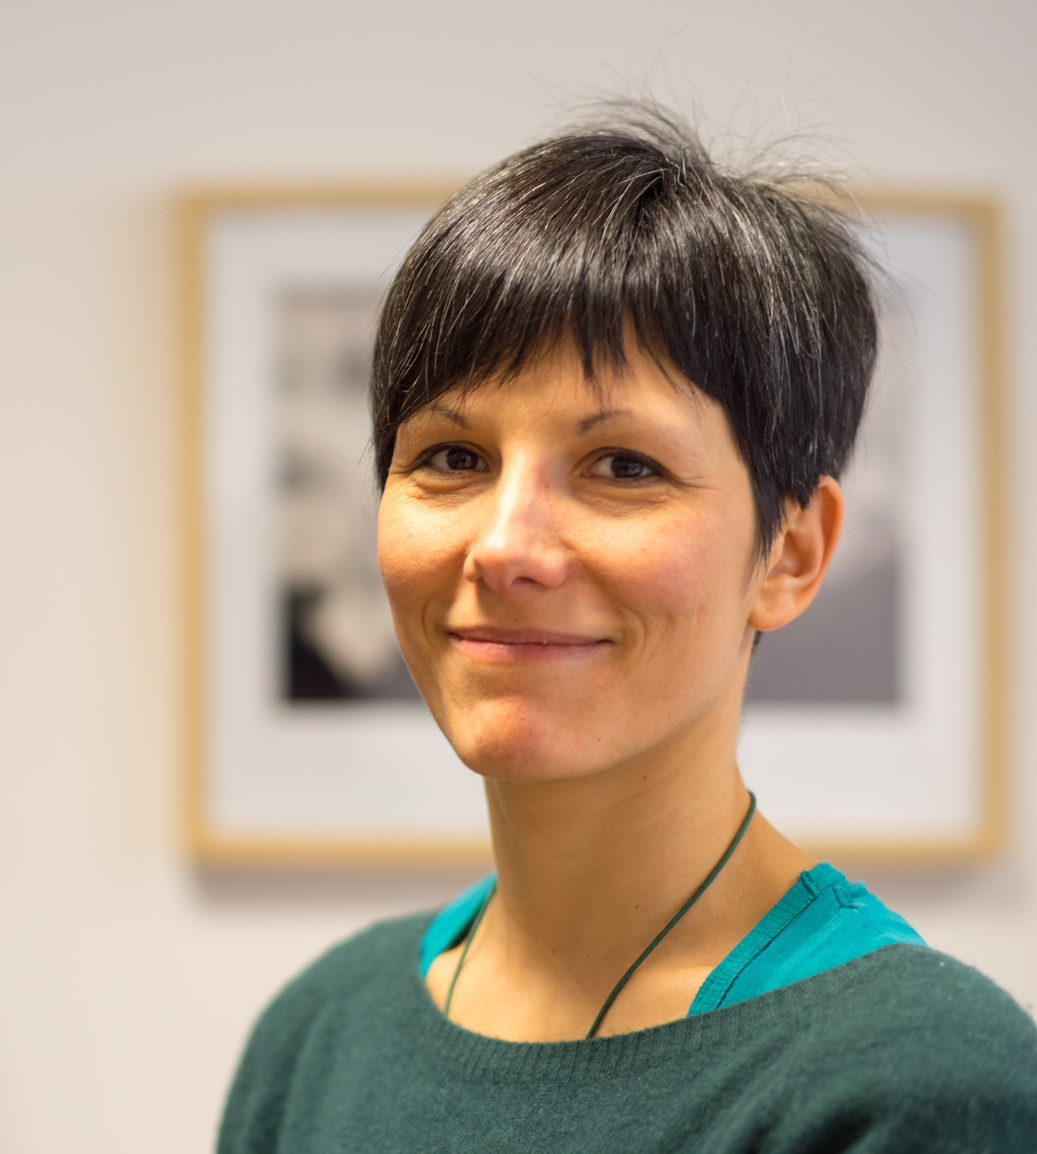
\includegraphics[width=1in,height=1.25in,clip,keepaspectratio]{Picture1.png}}]{Giulia Boato} is Associate Professor at the Department of Information Engineering and Computer Science (DISI) of the University of Trento (Italy). She is currently coordinating the Euregio project NOTIS Humans in a digital era – New Opportunities and Threats for Information Security.  She was co-chair of the International Workshop Living Web: making diversity a true asset within the International Semantic Web Conference 2009 and of the workshop on Event-based Media Integration and Processing co-located with ACM Multimedia Conference 2013. She was Technical Program Chair of the ACM Workshop on Information Hiding and Multimedia Security 2018. She is associate editor for the IEEE Transactions on Image Processing, for the ELSEVIER Signal Processing: Image Communication, and for the Journal of Electronic Imaging. Her research interests are focused on image and signal processing, with particular attention to multimedia data protection, data hiding and digital forensics, but also intelligent multidimensional data management and analysis. She is author of 120 papers in international conferences and journals, with H-index 22 (Google Scholar). She is elected member of the IEEE Multimedia Signal Processing Technical Committee (MMSP TC), of the IEEE Information Forensics and Security Technical Committee (IFS TC) and of the EURASIP Special Area Teams Biometrics, Data Forensics, and Security.
\end{IEEEbiography}

\begin{IEEEbiography}[{\includegraphics[width=1in,height=1.25in,clip,keepaspectratio]{a2.png}}]{Duc-Tien Dang-Nguyen} was born in Greenwich Village, New York, NY, USA in 
1977. He received the B.S. and M.S. degrees in aerospace engineering from 
the University of Virginia, Charlottesville, in 2001 and the Ph.D. degree in 
mechanical engineering from Drexel University, Philadelphia, PA, in 2008.

From 2001 to 2004, he was a Research Assistant with the Princeton Plasma 
Physics Laboratory. Since 2009, he has been an Assistant Professor with the 
Mechanical Engineering Department, Texas A{\&}M University, College Station. 
He is the author of three books, more than 150 articles, and more than 70 
inventions. His research interests include high-pressure and high-density 
nonthermal plasma discharge processes and applications, microscale plasma 
discharges, discharges in liquids, spectroscopic diagnostics, plasma 
propulsion, and innovation plasma applications. He is an Associate Editor of 
the journal \emph{Earth, Moon, Planets}, and holds two patents. 

Dr. Author was a recipient of the International Association of Geomagnetism 
and Aeronomy Young Scientist Award for Excellence in 2008, and the IEEE 
Electromagnetic Compatibility Society Best Symposium Paper Award in 2011. 
\end{IEEEbiography}

\begin{IEEEbiography}[{\includegraphics[width=1in,height=1.25in,clip,keepaspectratio]{a3.png}}]{Francesco G.B. De Natale} (M'87) received the B.S. degree in mechanical 
engineering from National Chung Cheng University, Chiayi, Taiwan, in 2004 
and the M.S. degree in mechanical engineering from National Tsing Hua 
University, Hsinchu, Taiwan, in 2006. He is currently pursuing the Ph.D. 
degree in mechanical engineering at Texas A{\&}M University, College 
Station, TX, USA.

From 2008 to 2009, he was a Research Assistant with the Institute of 
Physics, Academia Sinica, Tapei, Taiwan. His research interest includes the 
development of surface processing and biological/medical treatment 
techniques using nonthermal atmospheric pressure plasmas, fundamental study 
of plasma sources, and fabrication of micro- or nanostructured surfaces. 

Mr. Author's awards and honors include the Frew Fellowship (Australian 
Academy of Science), the I. I. Rabi Prize (APS), the European Frequency and 
Time Forum Award, the Carl Zeiss Research Award, the William F. Meggers 
Award and the Adolph Lomb Medal (OSA).
\end{IEEEbiography}

\EOD

\end{document}
